%----------------------------------------------------------------------------------------
%	PACKAGES AND OTHER DOCUMENT CONFIGURATIONS
%----------------------------------------------------------------------------------------

\documentclass{article}

\usepackage{fancyhdr} % Required for custom headers
\usepackage{lastpage} % Required to determine the last page for the footer
\usepackage{extramarks} % Required for headers and footers
\usepackage[usenames,dvipsnames]{color} % Required for custom colors
\usepackage{pgf} % Required to insert pgf plots from matplotlib
\usepackage{graphicx} % Required to insert images
\usepackage{listings} % Required for insertion of code
\usepackage{courier} % Required for the courier font
\usepackage{lipsum} % Used for inserting dummy 'Lorem ipsum' text into the template
\usepackage[utf8]{inputenc}
\usepackage[english]{babel}
\usepackage{subcaption, caption, tabularx, minted}
\usepackage{hyperref}

% Margins
\topmargin=-0.45in
\evensidemargin=0in
\oddsidemargin=0in
\textwidth=6.5in
\textheight=9.0in
\headsep=0.25in

\linespread{1.1} % Line spacing

% Set up the header and footer
\pagestyle{fancy}
%\lhead{\hmwkAuthorName} % Top left header
\chead{\hmwkClass\ : \hmwkTitle} % Top center head
\rhead{\firstxmark} % Top right header
\lfoot{\lastxmark} % Bottom left footer
\cfoot{} % Bottom center footer
\rfoot{Page\ \thepage\ of\ \protect\pageref{LastPage}} % Bottom right footer
\renewcommand\headrulewidth{0.4pt} % Size of the header rule
\renewcommand\footrulewidth{0.4pt} % Size of the footer rule

\setlength\parindent{0pt} % Removes all indentation from paragraphs

%----------------------------------------------------------------------------------------
%	CODE INCLUSION CONFIGURATION
%----------------------------------------------------------------------------------------

\definecolor{MyDarkGreen}{rgb}{0.0,0.4,0.0} % This is the color used for comments
\lstloadlanguages{Perl} % Load Perl syntax for listings, for a list of other languages supported see: ftp://ftp.tex.ac.uk/tex-archive/macros/latex/contrib/listings/listings.pdf
\lstset{language=Perl, % Use Perl in this example
        frame=single, % Single frame around code
        basicstyle=\small\ttfamily, % Use small true type font
        keywordstyle=[1]\color{Blue}\bf, % Perl functions bold and blue
        keywordstyle=[2]\color{Purple}, % Perl function arguments purple
        keywordstyle=[3]\color{Blue}\underbar, % Custom functions underlined and blue
        identifierstyle=, % Nothing special about identifiers                                         
        commentstyle=\usefont{T1}{pcr}{m}{sl}\color{MyDarkGreen}\small, % Comments small dark green courier font
        stringstyle=\color{Purple}, % Strings are purple
        showstringspaces=false, % Don't put marks in string spaces
        tabsize=5, % 5 spaces per tab
        %
        % Put standard Perl functions not included in the default language here
        morekeywords={rand},
        %
        % Put Perl function parameters here
        morekeywords=[2]{on, off, interp},
        %
        % Put user defined functions here
        morekeywords=[3]{test},
       	%
        morecomment=[l][\color{Blue}]{...}, % Line continuation (...) like blue comment
        numbers=left, % Line numbers on left
        firstnumber=1, % Line numbers start with line 1
        numberstyle=\tiny\color{Blue}, % Line numbers are blue and small
        stepnumber=5 % Line numbers go in steps of 5
}

% Creates a new command to include a perl script, the first parameter is the filename of the script (without .pl), the second parameter is the caption
\newcommand{\perlscript}[2]{
\begin{itemize}
\item[]\lstinputlisting[caption=#2,label=#1]{#1.pl}
\end{itemize}
}

%----------------------------------------------------------------------------------------
%	DOCUMENT STRUCTURE COMMANDS
%	Skip this unless you know what you're doing
%----------------------------------------------------------------------------------------

% Header and footer for when a page split occurs within a problem environment
\newcommand{\enterProblemHeader}[1]{
%\nobreak\extramarks{#1}{#1 continued on next page\ldots}\nobreak
%\nobreak\extramarks{#1 (continued)}{#1 continued on next page\ldots}\nobreak
}

% Header and footer for when a page split occurs between problem environments
\newcommand{\exitProblemHeader}[1]{
%\nobreak\extramarks{#1 (continued)}{#1 continued on next page\ldots}\nobreak
%\nobreak\extramarks{#1}{}\nobreak
}

\setcounter{secnumdepth}{0} % Removes default section numbers
\newcounter{homeworkProblemCounter} % Creates a counter to keep track of the number of problems

\newcommand{\homeworkProblemName}{}
\newenvironment{homeworkProblem}[1][Problem \arabic{homeworkProblemCounter}]{ % Makes a new environment called homeworkProblem which takes 1 argument (custom name) but the default is "Problem #"
\stepcounter{homeworkProblemCounter} % Increase counter for number of problems
\renewcommand{\homeworkProblemName}{#1} % Assign \homeworkProblemName the name of the problem
\section{\homeworkProblemName} % Make a section in the document with the custom problem count
%\enterProblemHeader{\homeworkProblemName} % Header and footer within the environment
}{
%\exitProblemHeader{\homeworkProblemName} % Header and footer after the environment
}

\newcommand{\problemAnswer}[1]{ % Defines the problem answer command with the content as the only argument
\noindent\framebox[\columnwidth][c]{\begin{minipage}{0.98\columnwidth}#1\end{minipage}} % Makes the box around the problem answer and puts the content inside
}

\newcommand{\homeworkSectionName}{}
\newenvironment{homeworkSection}[1]{ % New environment for sections within homework problems, takes 1 argument - the name of the section
\renewcommand{\homeworkSectionName}{#1} % Assign \homeworkSectionName to the name of the section from the environment argument
\subsection{\homeworkSectionName} % Make a subsection with the custom name of the subsection
%\enterProblemHeader{\homeworkProblemName\ [\homeworkSectionName]} % Header and footer within the environment
}{
%\enterProblemHeader{\homeworkProblemName} % Header and footer after the environment
}

%----------------------------------------------------------------------------------------
%	NAME AND CLASS SECTION
%----------------------------------------------------------------------------------------

\newcommand{\hmwkTitle}{Exercise\ \#2} % Assignment title
\newcommand{\hmwkDueDate}{Tuesday,\ May 5,\ 2015} % Due date
\newcommand{\hmwkClass}{Advanced Parallel Computing} % Course/class
\newcommand{\hmwkClassTime}{} % Class/lecture time
\newcommand{\hmwkClassInstructor}{} % Teacher/lecturer
\newcommand{\hmwkAuthorName}{Svend Dorkenwald, Günther Schindler} % Your name

%----------------------------------------------------------------------------------------
%	TITLE PAGE
%----------------------------------------------------------------------------------------

\title{
\vspace{2in}
\textmd{\textbf{\hmwkClass:\ \hmwkTitle}}\\
\normalsize\vspace{0.1in}\small{Due\ on\ \hmwkDueDate}\\
\vspace{0.1in}\large{\textit{\hmwkClassTime}}
\vspace{3in}
}

\author{\textbf{\hmwkAuthorName}}
\date{} % Insert date here if you want it to appear below your name

%----------------------------------------------------------------------------------------

\begin{document}

\maketitle

%----------------------------------------------------------------------------------------
%	TABLE OF CONTENTS
%----------------------------------------------------------------------------------------

%\setcounter{tocdepth}{1} % Uncomment this line if you don't want subsections listed in the ToC

\newpage
\tableofcontents
\newpage

%----------------------------------------------------------------------------------------
%	Reading
%----------------------------------------------------------------------------------------

\begin{homeworkProblem}[Reading]

\subsection{The Future of Microprocessors}

\subsection{Software and the Concurrency Revolution}
Sutter and Larus focus in this paper on the implications of concurrency for software. Concurrency was becoming more important since CPU manufactures were starting to produce multicore CPUs with often reduced clock speeds for each core. Besides performance they name and improvement of responsiveness by performing work asynchronously as second reason to program concurrently . \\
Their analyses leads to the conclusion that programmers are very likely to be overburdened by writing and debugging concurrent programs. Therefore, better tools need to be developed which itself is a difficult task. In terms of programming models they state that current models do not provide sufficient options to handle unstructered parallelism, specifically shared states. Especially locks introduce many new problems making them to a bad option. \\
The authors address important topics which even may have prevented the earlier introduction of multicore architectures. Although defining several features of better suited programming models and debugging tools they fail to give answers and ideas. Hence, this paper might only be helpful for outsiders and newbys to understand the predominant problem. \\
Nevertheless, we give this paper a week accept.\\

\end{homeworkProblem}

%----------------------------------------------------------------------------------------
%	Pointer Chasing Benchmark
%----------------------------------------------------------------------------------------

\begin{homeworkProblem}[Pointer Chasing Benchmark]


\end{homeworkProblem}

%----------------------------------------------------------------------------------------
%	Multi-threaded load bandwidth
%----------------------------------------------------------------------------------------

\begin{homeworkProblem}[Multi-threaded load bandwidth]

In this section we tested the performance of three devices: Creek08, Moore, ThinkPad E330 (8GB RAM). \\
Therefore, we loaded an amount of data with different numbers of threads from RAM and measured the time until the last thread finished. To increase the quality of the measurement we repeated each of them for five seconds and averaged the times. \\
For the first measurement we loaded 4MB per thread from RAM (\autoref{fig:bw_d}) and for the second 1GB in total (\autoref{fig:bw_c}). 

\begin{figure}[!ht]
	\centering
    \begin{subfigure}[l]{0.45\textwidth}
    	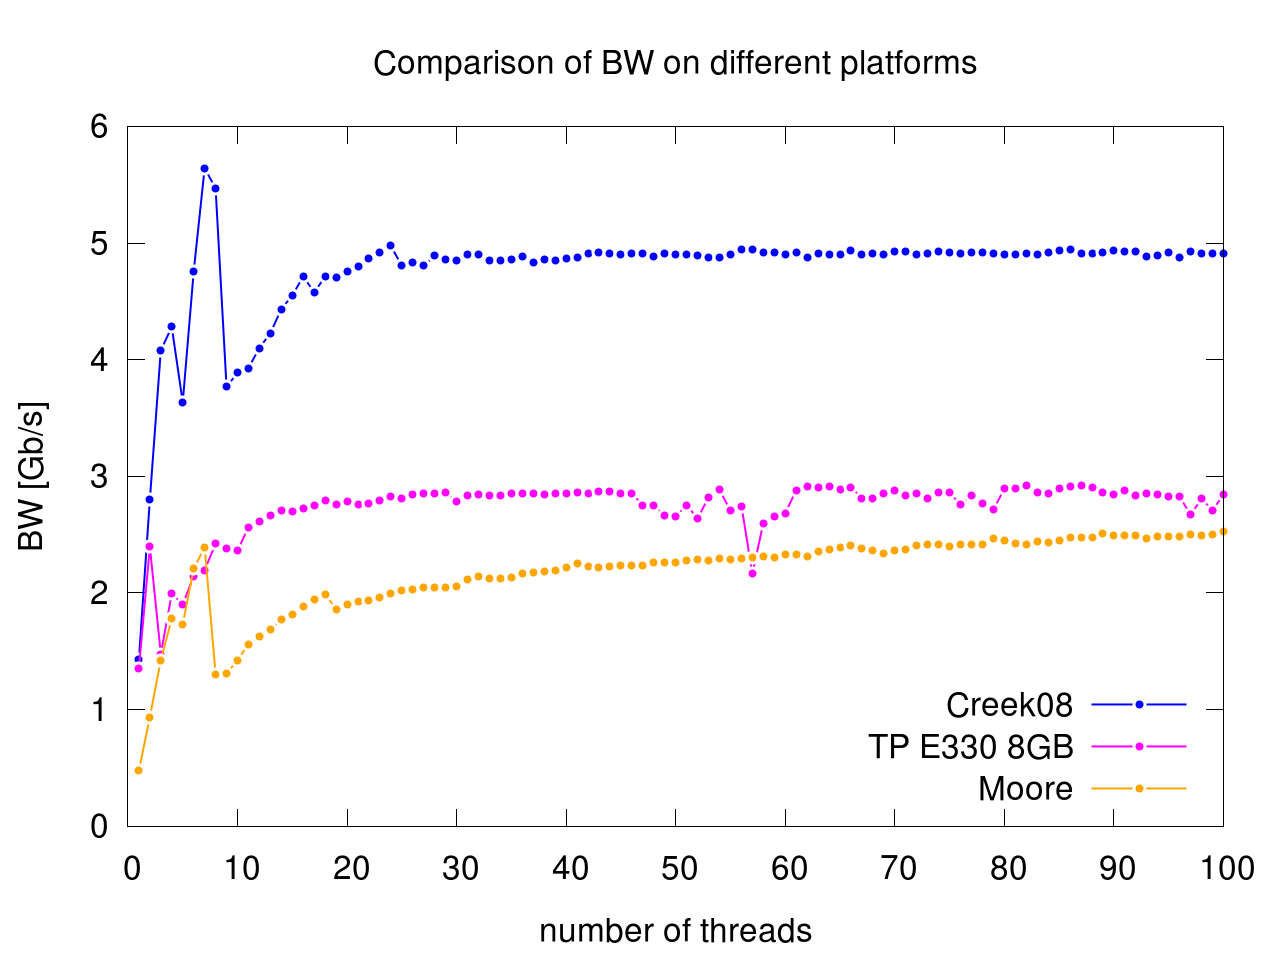
\includegraphics[width=\textwidth]{bw_d.png}
        \caption{Bandwidth comaprsion for loading 4MB per thread from RAM.}
        \label{fig:bw_d}
    \end{subfigure}
    \hfill
    \begin{subfigure}[r]{0.45\textwidth}
    	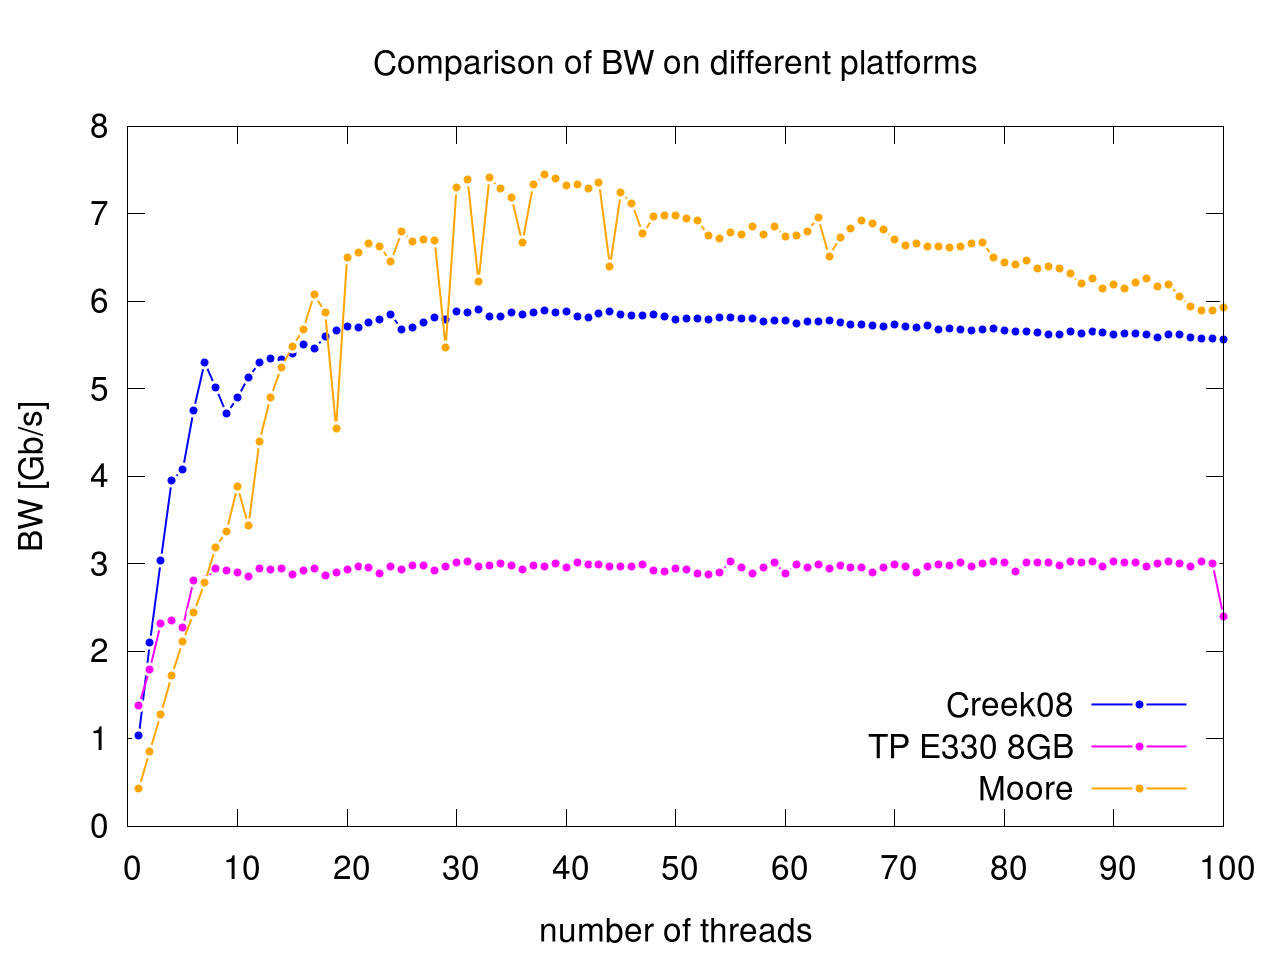
\includegraphics[width=\textwidth]{bw_c.png}
        \caption{Bandwidth comparison for loading 1GB from RAM.}
        \label{fig:bw_c}
    \end{subfigure}
\end{figure}

Surprisingly, Moore performs worse for the first scenario. It seems as if the bandwidth on Moore is highly dependable on the data size whereas this is barely not the case for the two other platforms. This is also supported by the decline of the BW-curve for Moore in \autoref{fig:bw_c}. In general the maximum bandwidths reported by Intel for the different platforms were not reached. Probably, the speed of the RAM slots is the main bottleneck. These theoretical numbers may also only be reached for very large data sizes.\\



\end{homeworkProblem}

\clearpage
\end{document}
